\begin{frame}{Parâmetros para moduladar a carga}
	\begin{itemize}
		\item \textbf{Tempo de planejamento de carga:} Um período de tempo em que a carga de trabalho é modulada, caracterizando a mudança do comportamento das requisições de maneira programada;
		
		\item \textbf{Tipo de modulação:} a modulação será apresentada conforme as funções ou sinais propostos por \cite{Hellerstein2004};
		
		\item \textbf{Tempo de interrupções:} Período de interrupções/pausa após o \textit{Tempo de planejamento de carga};
		
		\item \textbf{Quantidade de clientes na modulação:} reservar uma quantidade de clientes EBs, que estão com dedicação exclusiva para a modulação da carga.
	\end{itemize}	
\end{frame}

\begin{frame}{Possibilidade de cargas moduláveis pela extensão}
	\begin{columns}
		\column{0.5\textwidth}
		\begin{minipage}[c][0.4\textheight][c]{\linewidth}
			\centering
			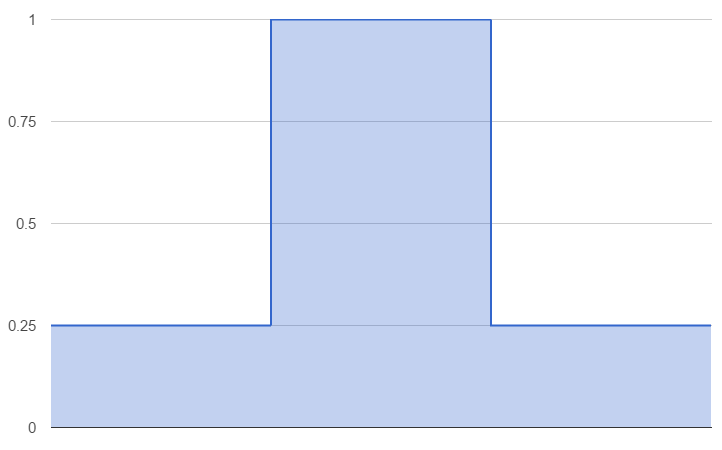
\includegraphics[width=0.8\linewidth]{../monograph/images/carga-sintetica1.png}
			\label{fig:degrau-positivo}
		\end{minipage}
		\begin{minipage}[c][0.4\textheight][c]{\linewidth}
			\centering
			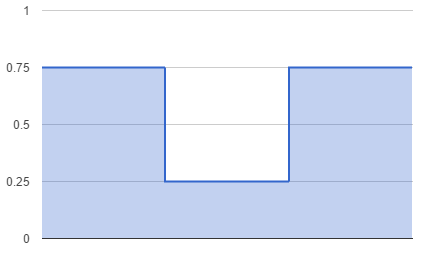
\includegraphics[width=0.8\linewidth]{../monograph/images/carga-sintetica2.png}
			\label{fig:degrau-negativo}
		\end{minipage}
		\column{0.5\textwidth}
		\begin{minipage}[c][0.4\textheight][c]{\linewidth}
			\begin{enumerate}
				\item Degrau positivo,
				\item Degrau negativo,
				\item Onda quadrada;
			\end{enumerate}
		\end{minipage}
		\begin{minipage}[c][0.4\textheight][c]{\linewidth}
			\centering
			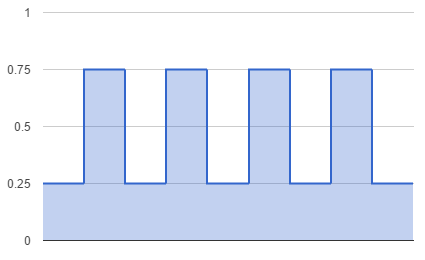
\includegraphics[width=0.8\linewidth]{../monograph/images/carga-sintetica3.png}
			\label{fig:onda-gradrada}
		\end{minipage}
	\end{columns}
\end{frame}

\begin{frame}{Arquitetura do experimento}
	\begin{columns}
		\column{0.4\textwidth}
		\begin{minipage}[c][0.4\textheight][c]{\linewidth}
			\centering
			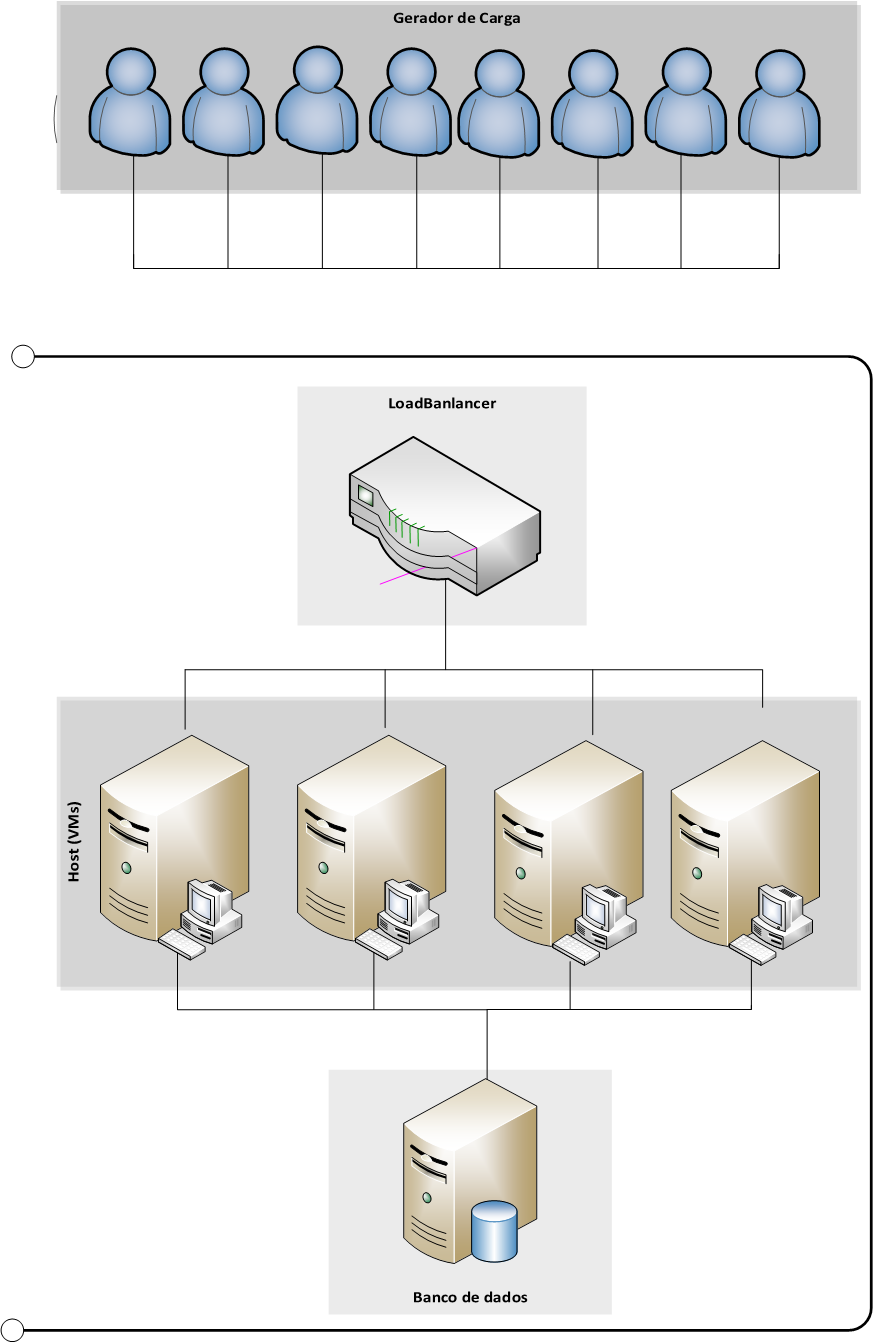
\includegraphics[scale=0.17]{../monograph/images/arquitetura-experimento.png}
			\label{fig:arquitetura-experimento}		
		\end{minipage}
		\column{0.6\textwidth}
		\begin{minipage}[c][0.4\textheight][c]{\linewidth}
			\begin{itemize}
				\item Gerador de Carga (\textit{Workload})
				\item Balanceador de carga (\textit{Load Balancer})
				\item Servidor Físico (\textit{Hypervisor})
				\item Servidor de dados (\textit{Data base})
			\end{itemize}
		\end{minipage}		
	\end{columns}
	
\end{frame}

\begin{frame}{Comportamento de métrica transiente}

\end{frame}

\begin{frame}{Comportamento de métrica transiente}
	\begin{columns}
		\column{0.45\textwidth}
		\begin{minipage}[c][0.45\textheight][c]{\linewidth}
			\centering
			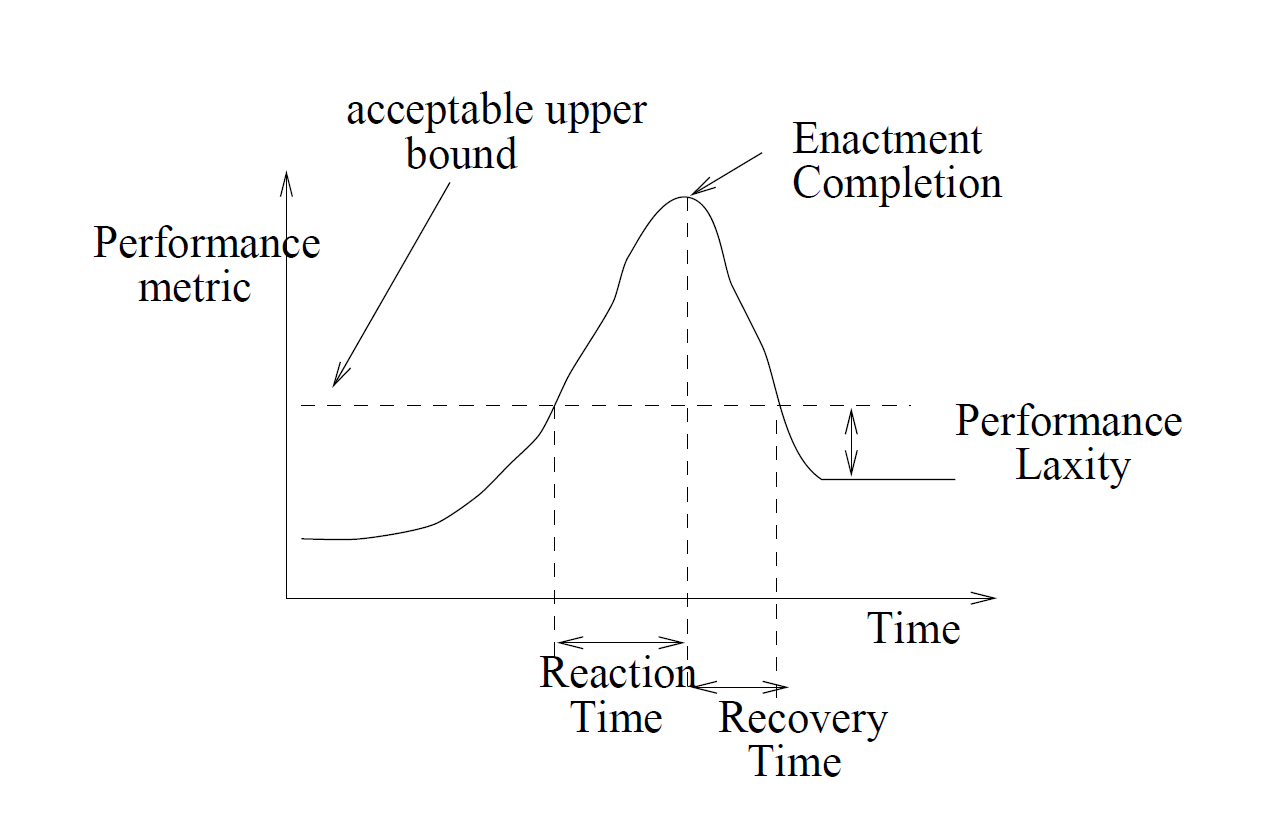
\includegraphics[width=1.27\linewidth]{../monograph/images/transient-metric.png}
			\label{fig:transient-metric}	
		\end{minipage}
		\column{0.55\textwidth}
		\begin{minipage}[c][0.55\textheight][c]{\linewidth}
			\begin{itemize}
				\item \textbf{\textit{Reaction Time} (Tempo de reação)} - o período entre a ocorrência da variação crítica e a conclusão da promulgação realocação de correção;
				
				\item \textbf{\textit{Recovery Time} (Tempo de Recuperação)} - o intervalo entre a conclusão, promulgação e da restauração de um nível de desempenho aceitável;
				
				\item \textbf{\textit{Performance Laxity} (Frouxidão performance)} - a diferença entre o \textit{required vs performance}, e o desempenho em estado estacionário, após a redistribuição;
			\end{itemize}
		\end{minipage}		
	\end{columns}
\end{frame}

\begin{frame}{Métrica transiente}
	\begin{itemize}
		\item \textbf{Conexões por segundo (\textit{Load Balancer}):} Conforme sugerido por \cite{Binnig2009}, medir a escalabilidade através do aumento dos interações web emitidos por segundo ao longo do tempo e de forma contínua contando a interação web que são respondidas em um intervalo de tempo de resposta,
		
		\item \textbf{Tempo de resposta (\textit{browsers}):} \cite{helder2014}, em um sistema dinâmico, cuja transformação entrada-saída não ocorre em tempo zero, mas é sujeita a uma inércia advinda dos processos físicos associados, possuí uma inércia intrínseca que atrasa o efeito que uma entrada terá na saída. Esses efeitos refletem no consequentemente nos comportamentos diversos que incluem retardo no tempo de resposta e possíveis oscilações; 	
	
	\end{itemize}
\end{frame}

\begin{frame}{Métrica transiente}
	\begin{itemize}
		\item \textbf{Taxa de utilização da CPU (VMs):} \cite{Nobile2013} afirma que diversas métricas podem ser analisadas para verificar o desempenho das máquinas virtuais, e cita alguns exemplos, como o tempo de inicialização, a taxa de utilização de CPU, o tempo médio de resposta e o \textit{throughput}, e usualmente, número de máquinas virtuais que hospedam serviços de interesse ao cliente e que respondem a uma carga de trabalho imposta por usuários através de requisições;
		
		\item \textbf{Taxa de utilização da CPU:} O trabalho apresentado por \cite{wang2009}, que lida com uma carga de trabalho variante no tempo e intensiva, demonstra que a CPU e I/O podem ser utilizadas para prever as necessidades dos recursos de um banco de dados e para orientar a alocação de recursos \textit{on-demand} de acordo com a exigência de carga de trabalho. Entretanto iremos somente considerar em nossos experimento a taxa de utilização do banco de dados.
	\end{itemize}
\end{frame}

\begin{frame}
	PEGAR IMAGEM DO EDWIN QUE EXPLICA A RESERVAR DOS EBs
\end{frame}

